% Created 2026-09-19 Sat 12:23
% Intended LaTeX compiler: pdflatex
\documentclass[10pt, a4paper]{article}
\usepackage[utf8]{inputenc}
\usepackage[T1]{fontenc}
\usepackage{graphicx}
\usepackage{longtable}
\usepackage{wrapfig}
\usepackage{rotating}
\usepackage[normalem]{ulem}
\usepackage{amsmath}
\usepackage{amssymb}
\usepackage{capt-of}
\usepackage{hyperref}
\usepackage[T1]{fontenc}
\usepackage[utf8]{inputenc}
\usepackage[a4paper]{geometry}
\geometry{verbose, tmargin=1.5cm, bmargin=1.5cm, lmargin=1.5cm, rmargin=1.5cm}
\author{Departamento de Matemáticas}
\date{\today}
\title{Matemáticas II}
\hypersetup{
 pdfauthor={Departamento de Matemáticas},
 pdftitle={Matemáticas II},
 pdfkeywords={},
 pdfsubject={},
 pdfcreator={Emacs 30.2 (Org mode 9.7.29)}, 
 pdflang={English}}
\begin{document}

\maketitle
\section{Límites y continuidad}
\label{sec:org8152f97}
\subsection{Ejemplo}
\label{sec:org60cb381}
\begin{center}
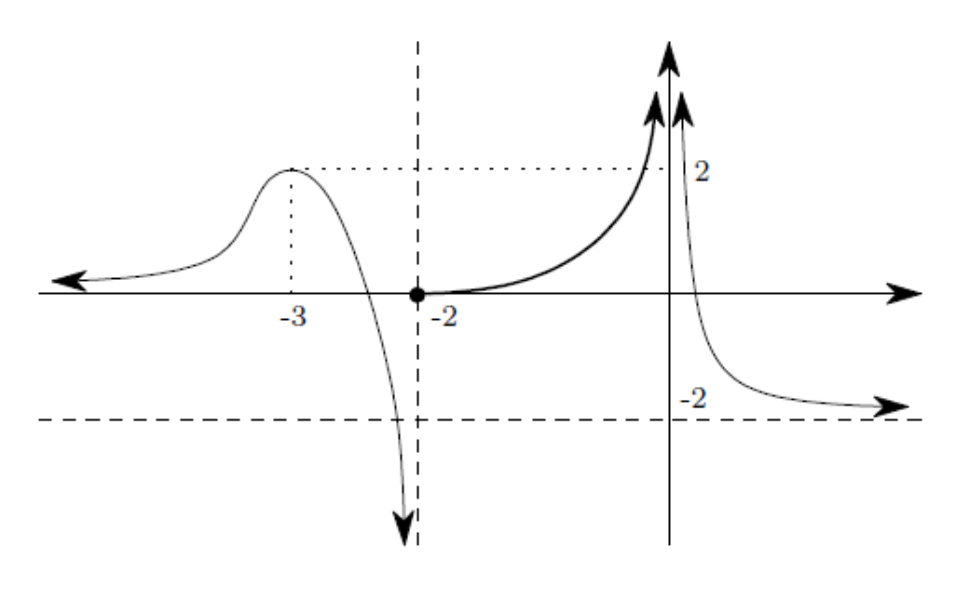
\includegraphics[width=.9\linewidth]{./_img/ejercicio001g.png}
\end{center}

\begin{itemize}
\item \(\displaystyle\lim_{ {x} \rightarrow {-\infty} } {f}\)
\item \(\displaystyle\lim_{ {x} \rightarrow {-3} } {f}\)
\item \(\displaystyle\lim_{ {x} \rightarrow {-2^-} } {f}\)
\end{itemize}
\begin{itemize}
\item \(\displaystyle\lim_{ {x} \rightarrow {-2^+} } {f}\)
\item \(\displaystyle\lim_{ {x} \rightarrow {-2} } {f}\)
\item \(\displaystyle\lim_{ {x} \rightarrow {0} } {f}\)
\item \(\displaystyle\lim_{ {x} \rightarrow {\infty} } {f}\)
\end{itemize}
\subsection{Ejemplo}
\label{sec:org70d22af}
Dibuja la gráfica de una función \(f\) tal que:

$$\begin{array}{|l|l|} \hline
\text{dom }f=\mathbb{R}-(-2,2)&\displaystyle\lim_{ {x} \rightarrow {-4} } {f}=-3 \\ \hline f(-2)=f(2)=0 & \displaystyle\lim_{ {x} \rightarrow {-\infty} } {f}=\infty \\ \hline f(-4)=-2 & \displaystyle\lim_{ {x} \rightarrow {\infty} } {f}=-2  \\ \hline\end{array}$$
\subsection*{Tareas}
\label{sec:org5f6c266}
\begin{itemize}
\item Estudiar:
\begin{itemize}
\item Concepto de límite finito o infinito (en un punto, laterales, en el infinito).
\item Teorema de existencia del límite.
\end{itemize}
\item Encuentra un ejemplo de que cada uno de los tipos de límite (finito en un punto, infinito en un punto, no exitente en un punto, lateral finito, lateral infinito,\ldots{}).
\item Ejercicios: \hyperref[sec:org64858d3]{1.3} - \hyperref[sec:org96e4bc2]{1.16}
\end{itemize}
\subsection{Ejercicio}
\label{sec:org64858d3}
Calcula las derivadas de las funciones siguientes:

\begin{itemize}
\item \(f(x) = \dfrac{x^3-2x^2+x}{(x-1)^2}\)
\item \(f(x) = x \cdot \sin^2 x\)
\item \(f(x) = \ln \left( \sqrt{1 - x^2} \right)\)
\item \(f(x) = \sqrt{\text{atan } \left( x^2 + 1 \right)}\)
\end{itemize}
\subsection{Ejercicio}
\label{sec:orgcdfe1b0}
\begin{center}
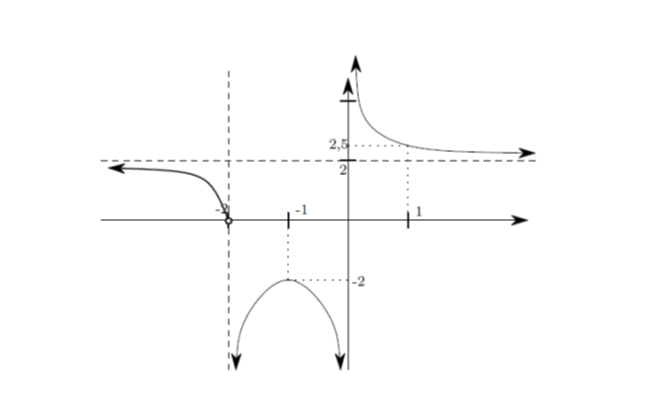
\includegraphics[width=.9\linewidth]{./_img/ejercicio0001a.png}
\end{center}

\begin{itemize}
\item \(\displaystyle\lim_{ {x} \rightarrow {-\infty} } {f}\)
\item \(\displaystyle\lim_{ {x} \rightarrow {-2} } {f}\)
\item \(\displaystyle\lim_{ {x} \rightarrow {-1} } {f}\)
\end{itemize}
\begin{itemize}
\item \(\displaystyle\lim_{ {x} \rightarrow {0} } {f}\)
\item \(\displaystyle\lim_{ {x} \rightarrow {1} } {f}\)
\item \(\displaystyle\lim_{ {x} \rightarrow {\infty} } {f}\)
\end{itemize}
\subsection{Ejercicio}
\label{sec:orgf4240b0}
\begin{center}
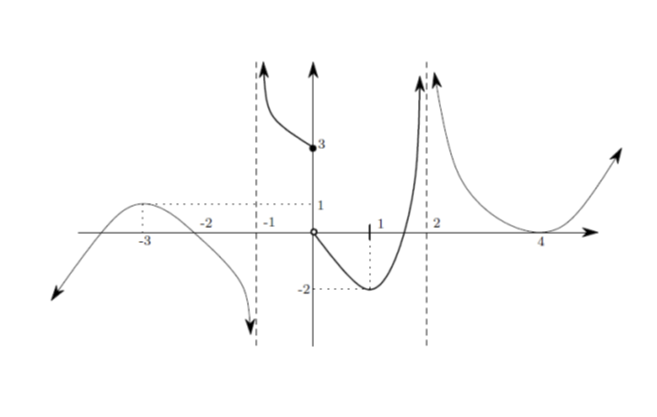
\includegraphics[width=.9\linewidth]{./_img/ejercicio0001b.png}
\end{center}

\begin{itemize}
\item \(\displaystyle\lim_{ {x} \rightarrow {-\infty} } {g}\)
\item \(\displaystyle\lim_{ {x} \rightarrow {-3} } {g}\)
\item \(\displaystyle\lim_{ {x} \rightarrow {-1} } {g}\)
\item \(\displaystyle\lim_{ {x} \rightarrow {0} } {g}\)
\end{itemize}
\begin{itemize}
\item \(\displaystyle\lim_{ {x} \rightarrow {1} } {g}\)
\item \(\displaystyle\lim_{ {x} \rightarrow {2} } {g}\)
\item \(\displaystyle\lim_{ {x} \rightarrow {\infty} } {g}\)
\end{itemize}
\subsection{Ejercicio}
\label{sec:org67268d2}
\begin{center}
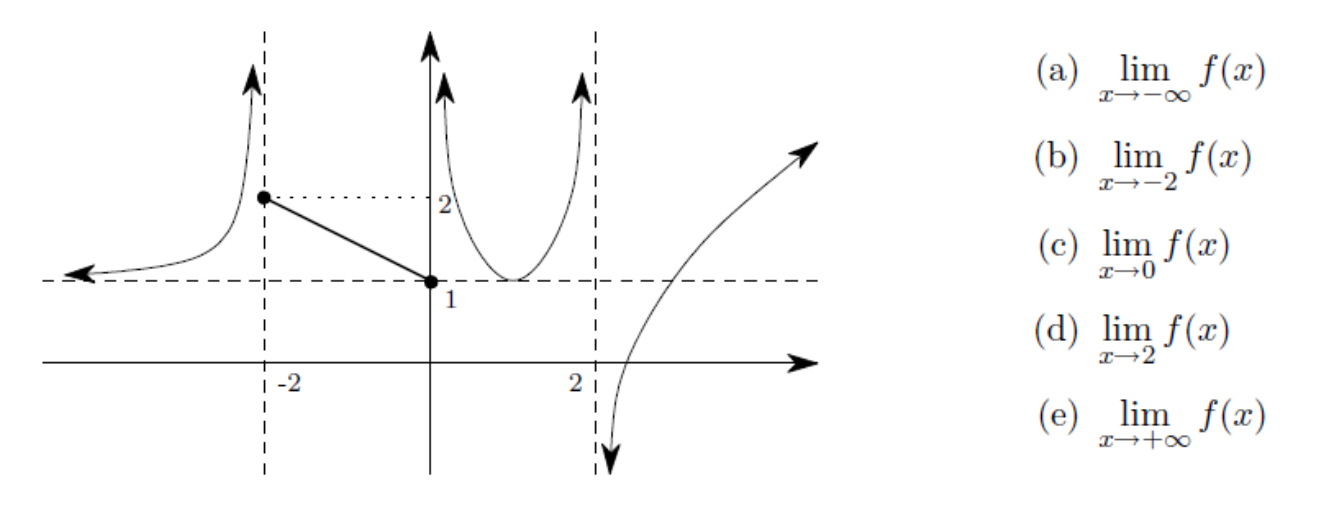
\includegraphics[width=.9\linewidth]{./_img/ejercicio001c.png}
\end{center}
\subsection{Ejercicio}
\label{sec:org86c35f0}
\begin{center}
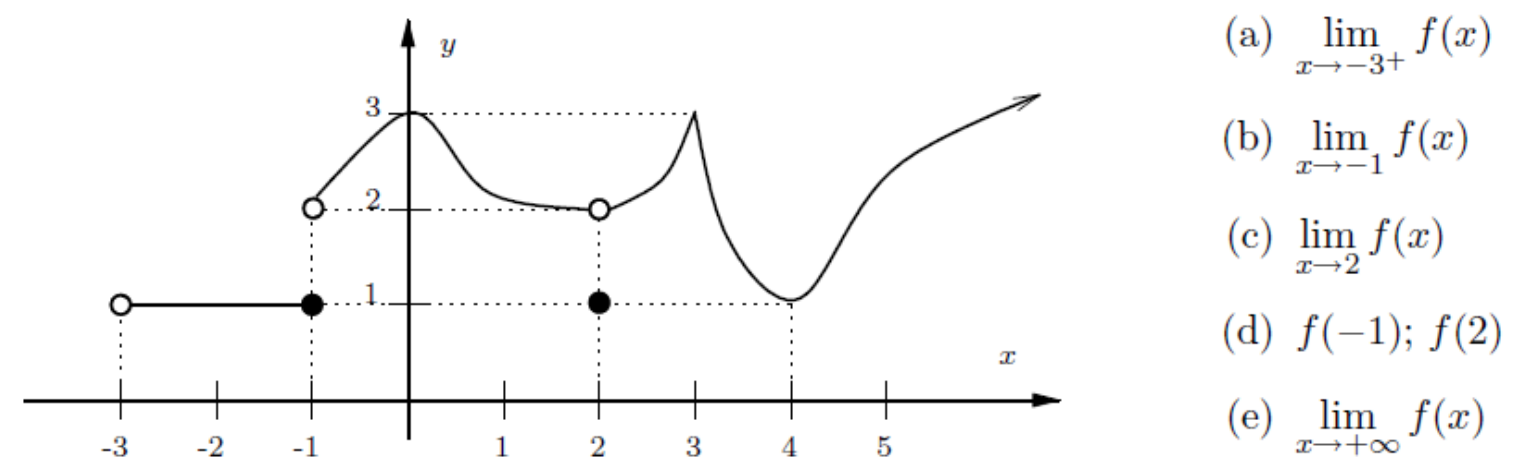
\includegraphics[width=.9\linewidth]{./_img/ejercicio001d.png}
\end{center}
\subsection{Ejercicio}
\label{sec:org0958e23}
\begin{center}
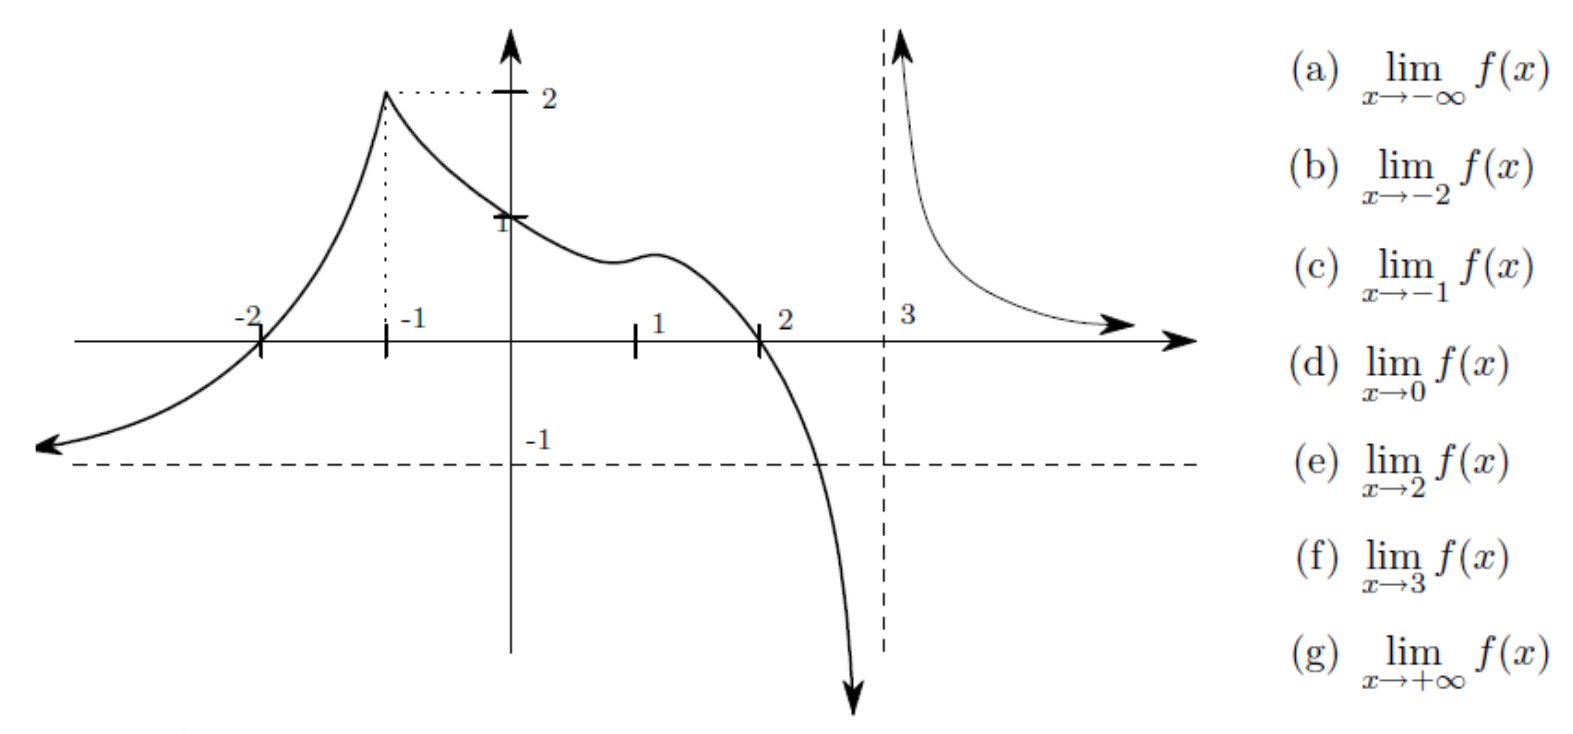
\includegraphics[width=.9\linewidth]{./_img/ejercicio001e.png}
\end{center}
\subsection{Ejercicio}
\label{sec:org44b8ceb}
\begin{center}
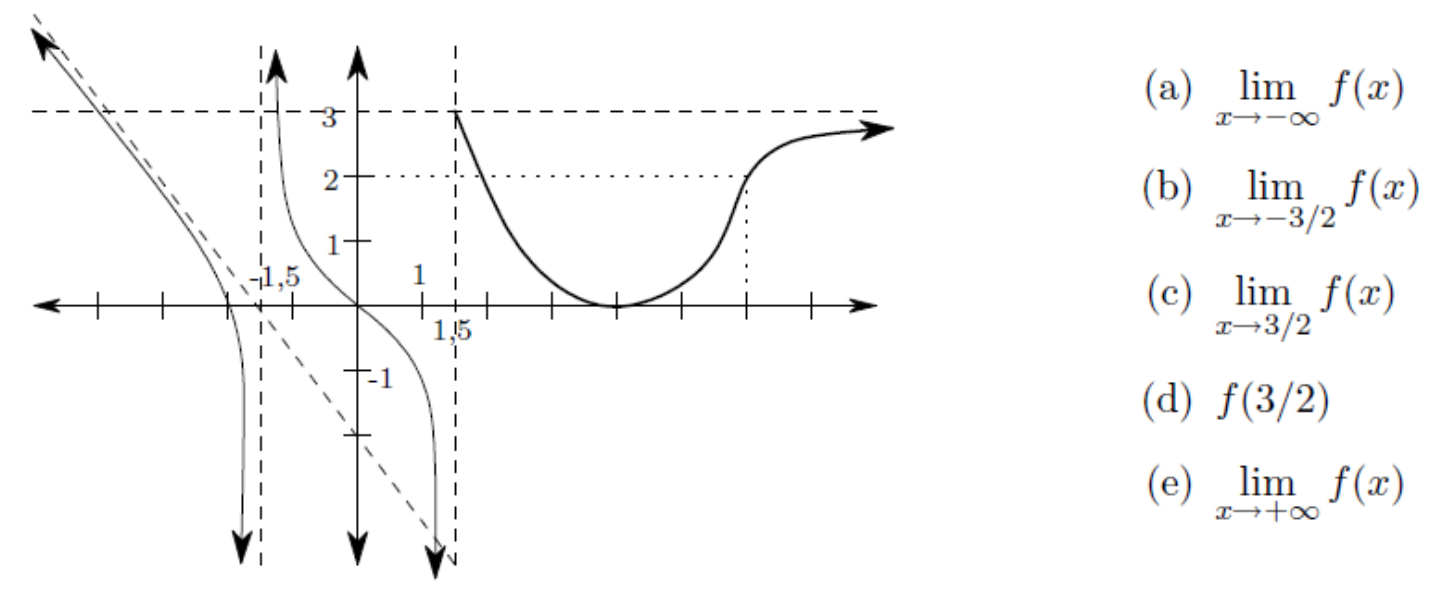
\includegraphics[width=.9\linewidth]{./_img/ejercicio001f.png}
\end{center}
\subsection{Ejercicio}
\label{sec:org9777da5}
Dibuja la gráfica de una función \(f\) tal que:

$$\begin{array}{|l|l|l|} \hline
\text{dom }h=\mathbb{R}-\{-2,2\}&h(-3)=1&\displaystyle\lim_{ {x} \rightarrow {2^-} } {h}=-\infty\\ \hline
\displaystyle\lim_{ {x} \rightarrow {-\infty} } {h}=-\infty&\displaystyle\lim_{ {x} \rightarrow {-2^-} } {h}=-\infty&\displaystyle\lim_{ {x} \rightarrow {2^+} } {h}=\infty\\ \hline
\displaystyle\lim_{ {x} \rightarrow {-3} } {h}=-2&\displaystyle\lim_{ {x} \rightarrow {-2^+} } {h}=\infty&\displaystyle\lim_{ {x} \rightarrow {\infty} } {h}=\infty\\ \hline\end{array}$$
\subsection{Ejercicio}
\label{sec:org1e3dfe8}
Dibuja la gráfica de una función \(f\) tal que:

\begin{center}
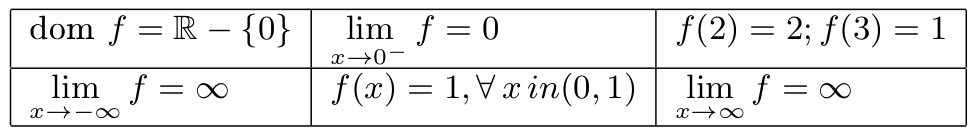
\includegraphics[width=.9\linewidth]{./_img/ejercicio002b.png}
\end{center}
\subsection{Ejercicio}
\label{sec:orgac289ca}
Dibuja la gráfica de una función \(f\) tal que:

\begin{center}
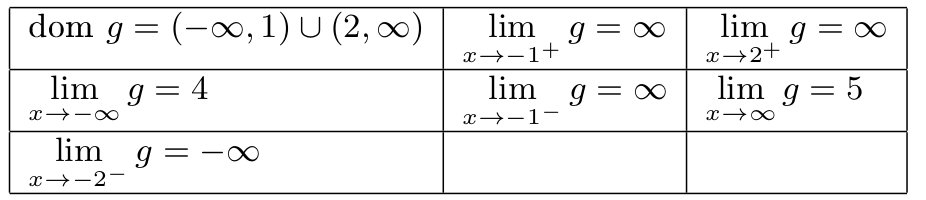
\includegraphics[width=.9\linewidth]{./_img/ejercicio002c.png}
\end{center}
\subsection{Ejercicio}
\label{sec:org842bc1d}
Dibuja la gráfica de una función \(f\) tal que:

\begin{center}
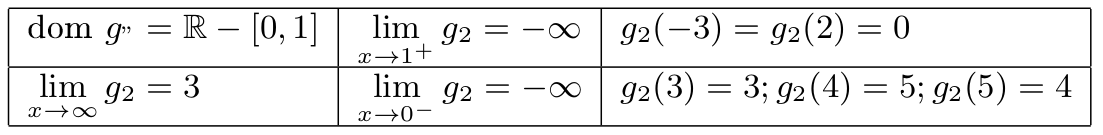
\includegraphics[width=.9\linewidth]{./_img/ejercicio002e.png}
\end{center}
\subsection{Ejercicio}
\label{sec:org27ccf7f}
Dibuja la gráfica de una función \(f\) tal que:

\begin{center}
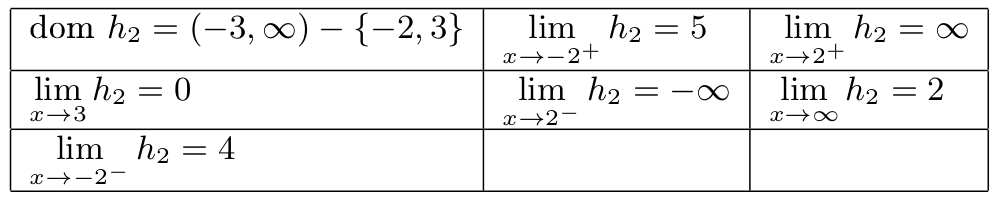
\includegraphics[width=.9\linewidth]{./_img/ejercicio002f.png}
\end{center}
\subsection{Ejercicio}
\label{sec:org391119f}
Dibuja la gráfica de una función \(f\) tal que:

\begin{center}
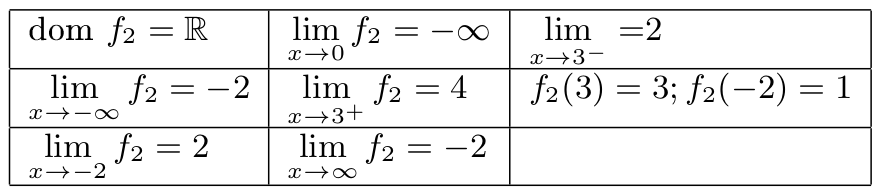
\includegraphics[width=.9\linewidth]{./_img/ejercicio002g.png}
\end{center}
\subsection{Ejercicio}
\label{sec:org96e4bc2}
Dibuja la gráfica de una función \(f\) tal que:

\begin{center}
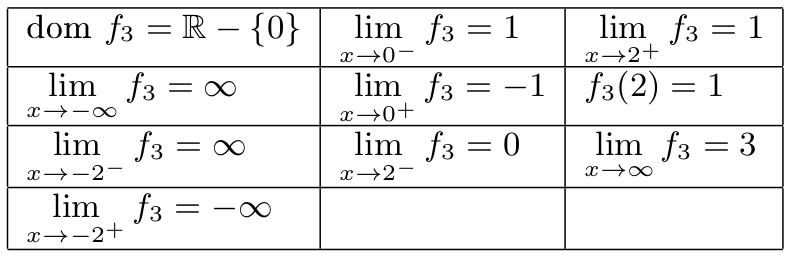
\includegraphics[width=.9\linewidth]{./_img/ejercicio002h.png}
\end{center}
\subsection{Ejemplo}
\label{sec:orgebdcbd7}
Sea \(f\) una función de la que se sabe que:

\begin{itemize}
\item \(\text{dom} f =\mathbb{R}\);
\item \(f(1)=0\);
\item \(\displaystyle\lim_{ {x} \rightarrow {1^-} } {f} = \infty\); \(\displaystyle\lim_{ {x} \rightarrow {1^+} } {f}=-\infty\); y,
\item \(\displaystyle\lim_{ {x} \rightarrow {-\infty} } {f}=\displaystyle\lim_{ {x} \rightarrow {\infty} } {f}=2\).
\end{itemize}


\begin{enumerate}
\item Determine razonadamente o discuta la inexistencia del límite siguiente: \(\displaystyle\lim_{ {x} \rightarrow {1} } {f^2}\).
\item Calcule \(\displaystyle\lim_{ {x} \rightarrow {1} } {(f \circ f)}\) (sugerencia: calcule primero los límites laterales).
\end{enumerate}
\subsection*{Tareas}
\label{sec:org11163eb}
\begin{itemize}
\item Estudiar: límites de funciones elementales en su dominio.
\item Estudiar: límites de operaciones (\(+\), \(\cdot\), \(/\), \(\circ\)).
\item Estudiar: límites de funciones a trozos
\item Ejercicios: 1.17, 1.18.
\end{itemize}
\subsection{Ejercicio}
\label{1.17}
\begin{center}
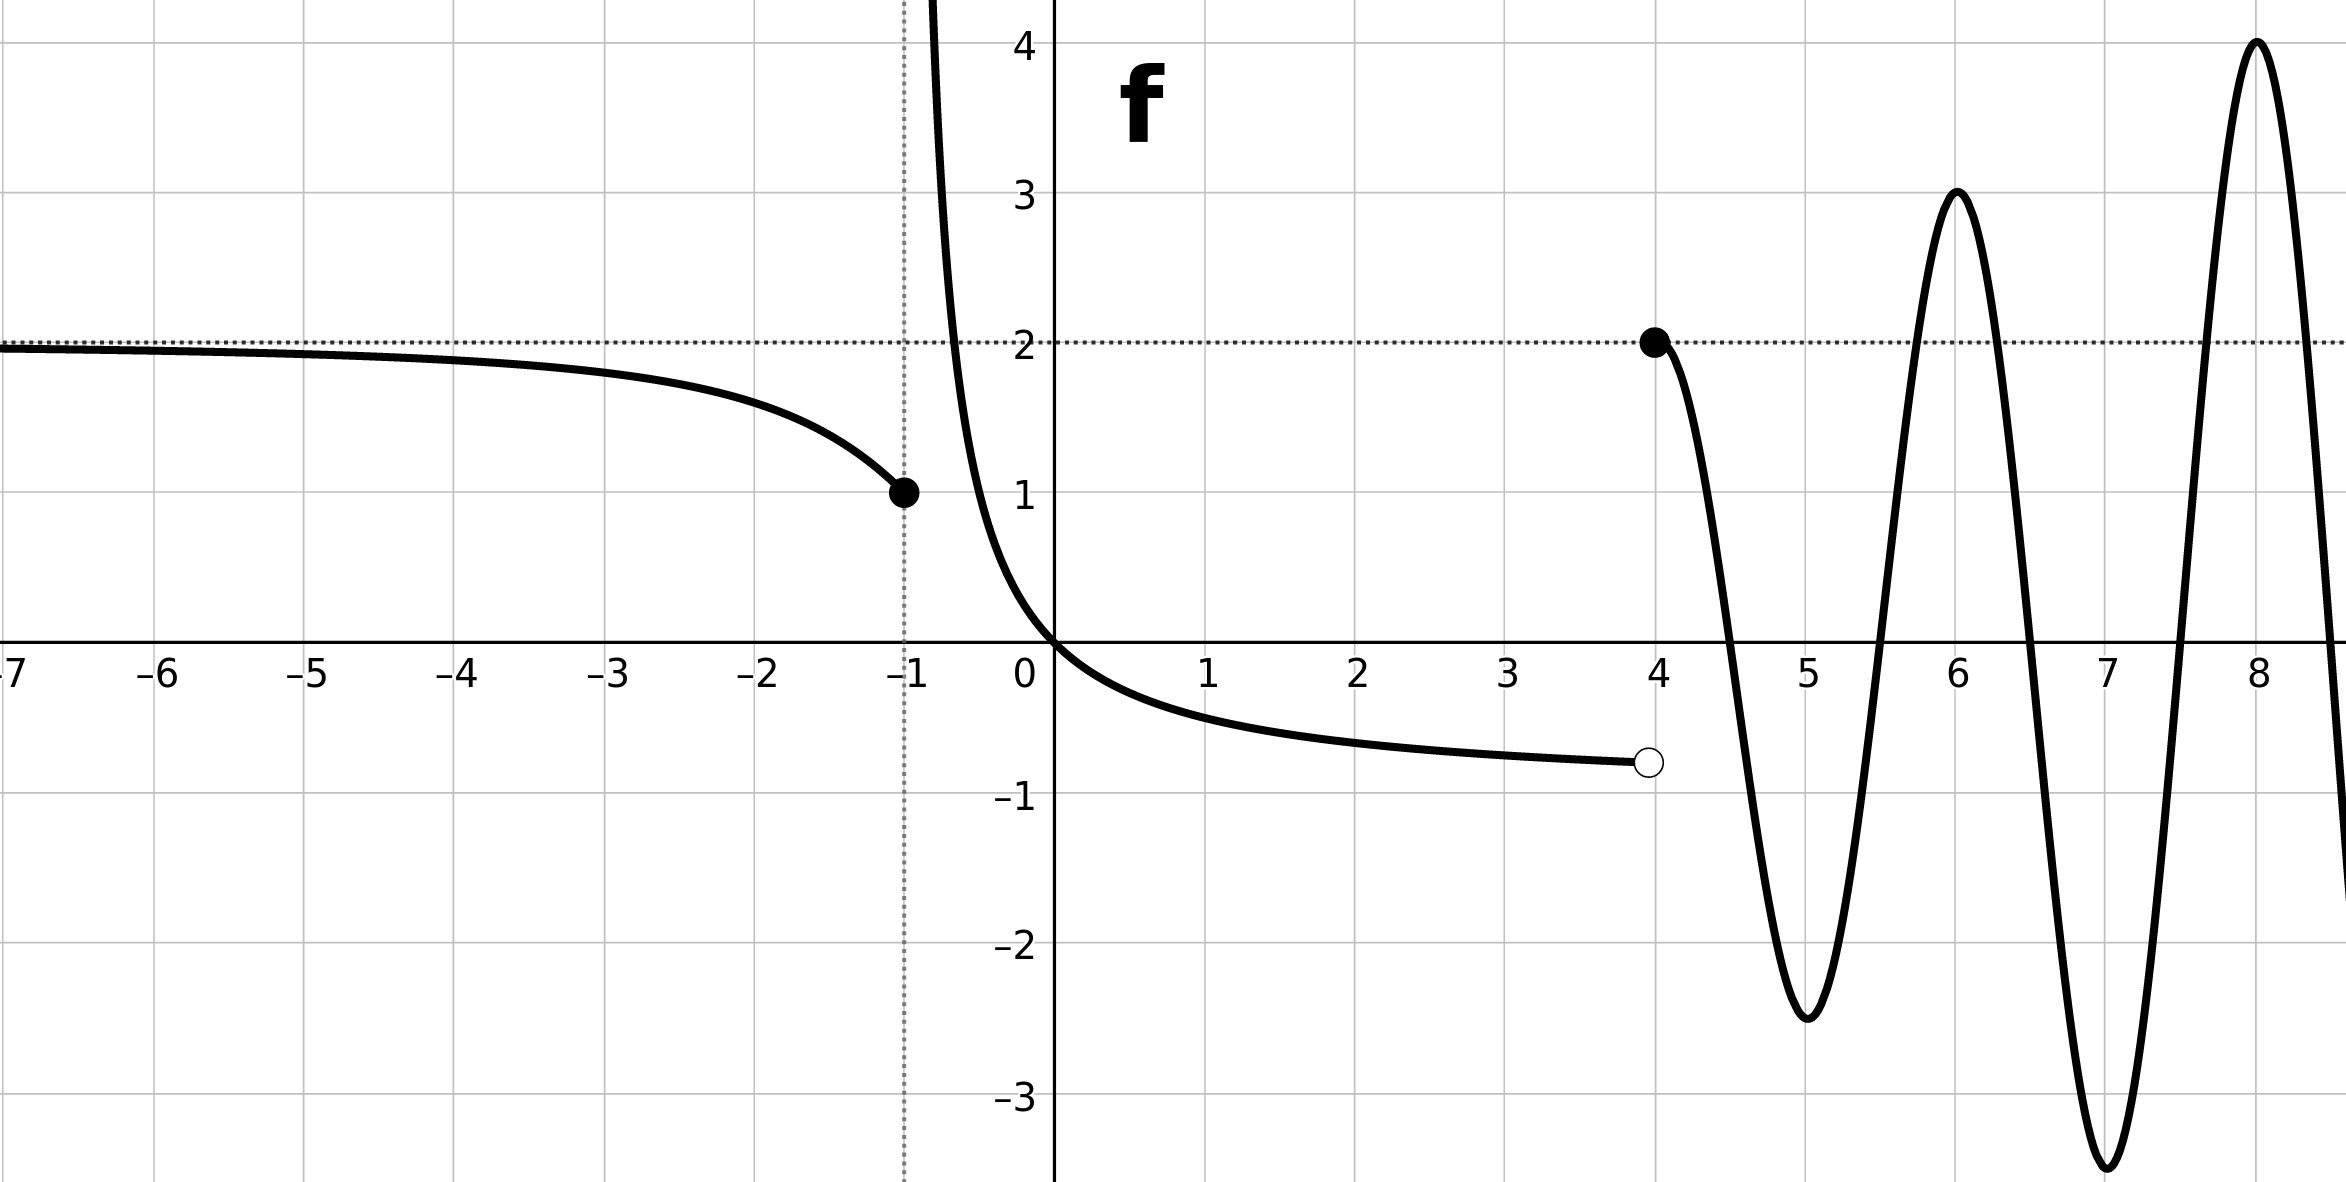
\includegraphics[width=.9\linewidth]{./_img/f3.png}
\end{center}
\begin{center}
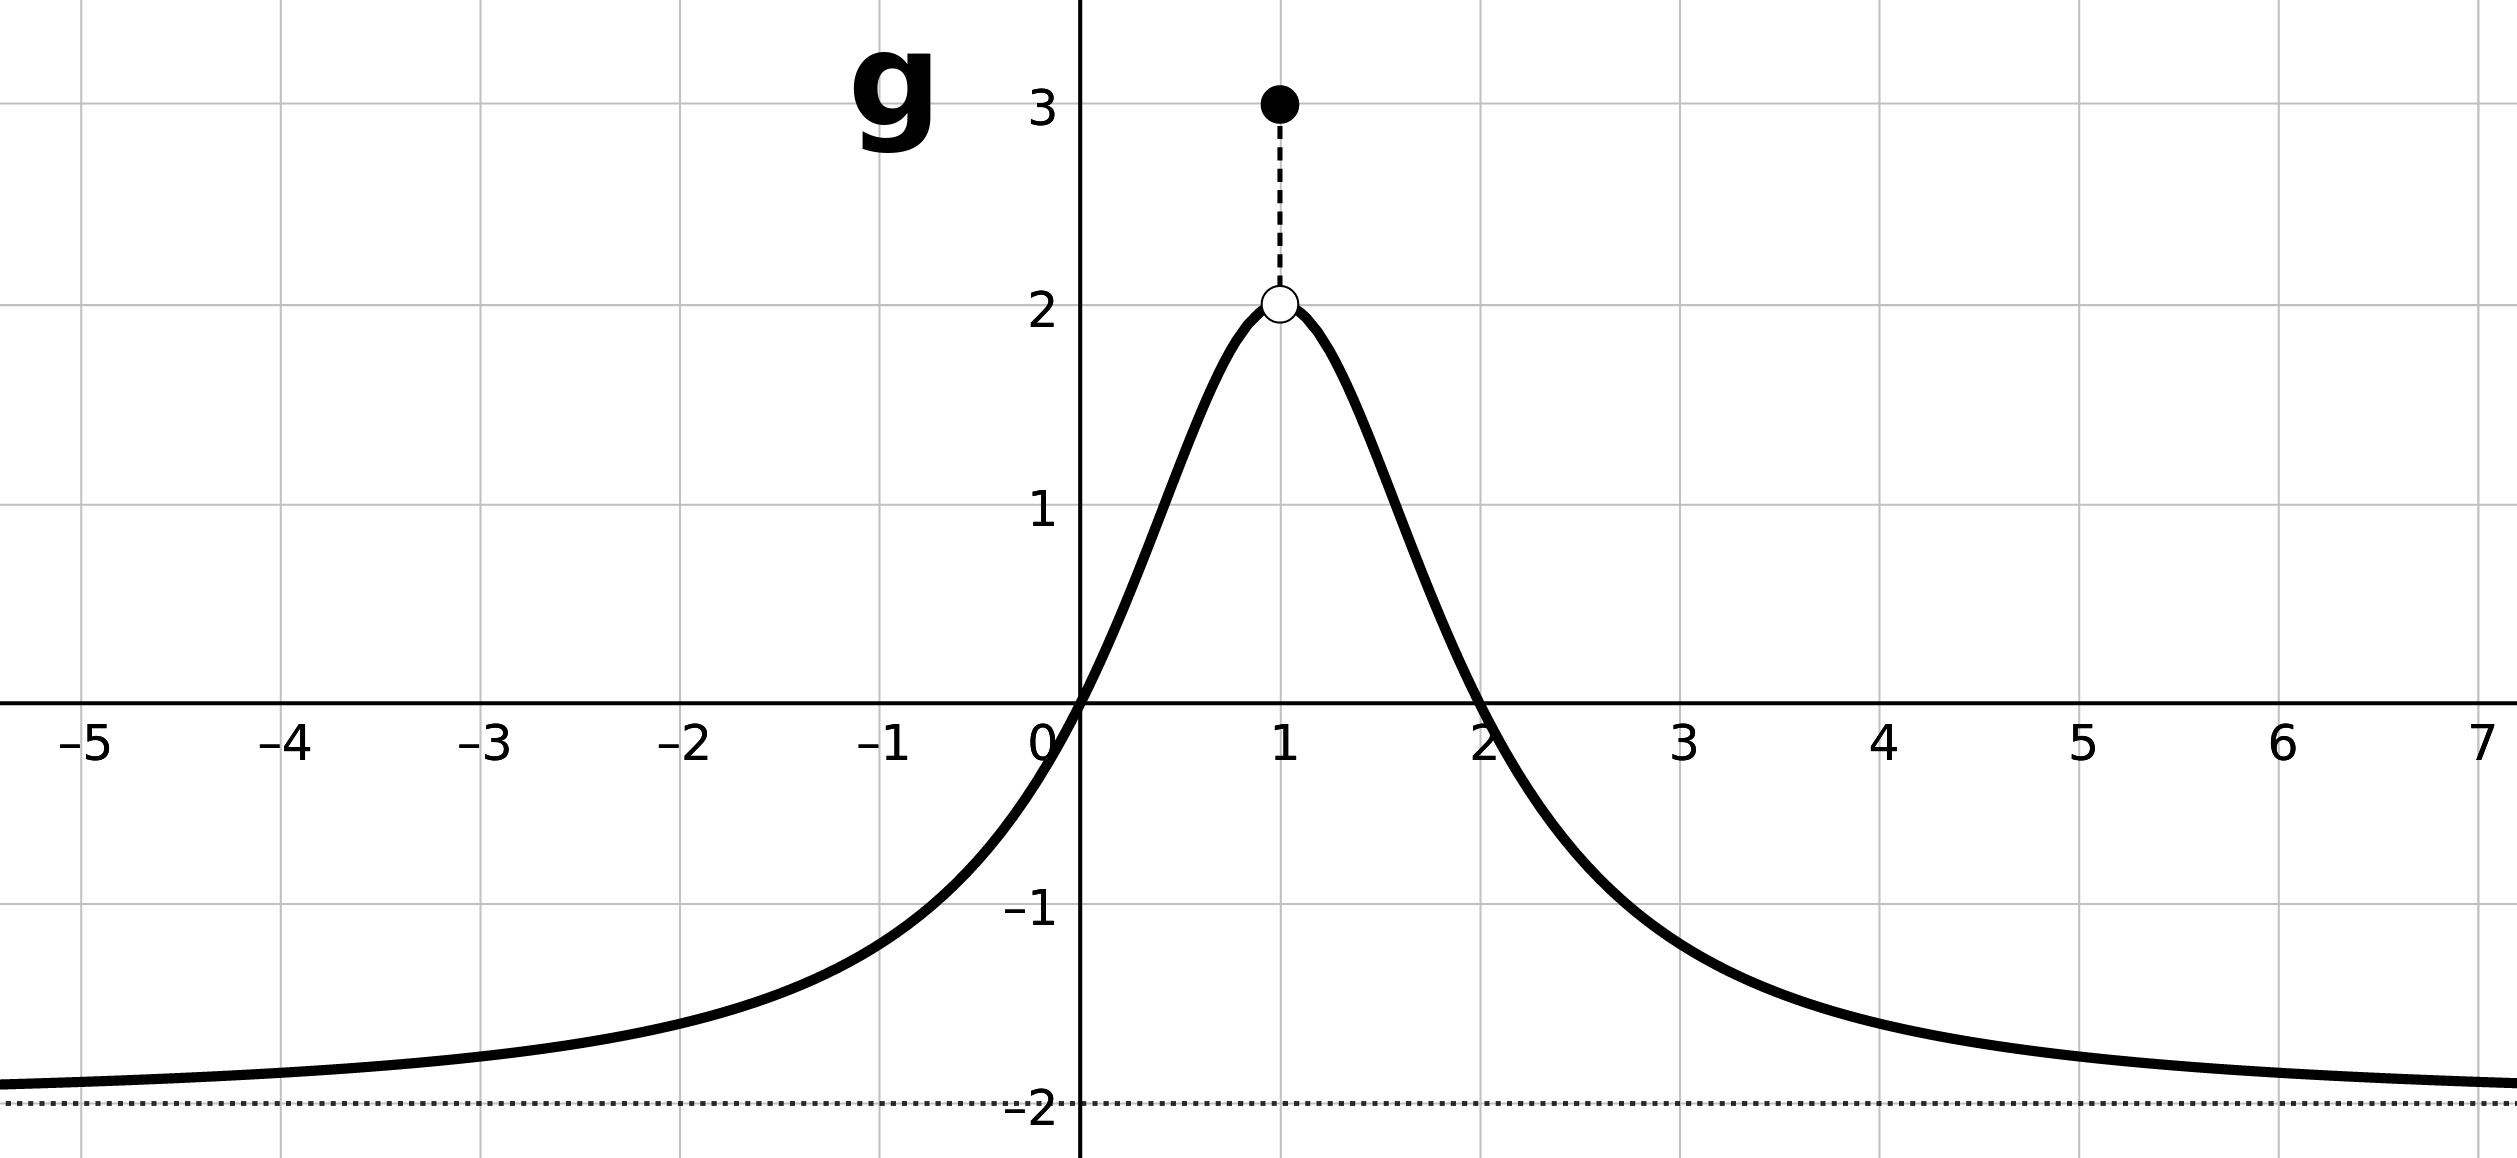
\includegraphics[width=.9\linewidth]{./_img/g3.png}
\end{center}
\begin{itemize}
\item \(\displaystyle\lim_{ {x} \rightarrow {-1} } {f}\), \(\displaystyle\lim_{ {x} \rightarrow {4} } {f}\) y \(\displaystyle\lim_{ {x} \rightarrow {1} } {g}\)
\item \(\displaystyle\lim_{ {x} \rightarrow {-\infty} } {(f+g)}\)
\item \(\displaystyle\lim_{ {x} \rightarrow {-1^-} } {(g \circ f)}\)
\end{itemize}
\subsection*{Ejemplo}
\label{sec:org513e08c}
\begin{itemize}
\item \(\displaystyle\lim_{ {x} \rightarrow {-\infty} } {\left( x^3+10x^2+1 \right)}\)
\item \(\displaystyle\lim_{ {x} \rightarrow {\pi^-} } {\ln \left(\sin x\right)}\)
\item \(\displaystyle\lim_{ {x} \rightarrow {\infty} } {\left( \dfrac{1}{2} \right)^{x^2-x}}\)
\end{itemize}
\begin{itemize}
\item \(\displaystyle\lim_{ {x} \rightarrow {0^-} } {\dfrac{1}{1-e^{1/x}}}\)
\item \(\displaystyle\lim_{ {x} \rightarrow {0^+} } {\dfrac{1}{1-e^{1/x}}}\)
\item \(\displaystyle\lim_{ {x} \rightarrow {0^+} } {\dfrac{1}{1-e^{1/x}}}\)
\end{itemize}
\subsection{Ejercicio}
\label{1.18}
\begin{itemize}
\item \(\displaystyle\lim_{ {x} \rightarrow {1^+} } {\sqrt{\dfrac{x-1}{x+2}}}\)
\item \(\displaystyle\lim_{ {x} \rightarrow {1^-} } {\sqrt{\dfrac{x-1}{x+2}}}\)
\item \(\displaystyle\lim_{ {x} \rightarrow {2^+} } {\ln\left(\dfrac{x}{-2+x}\right)}\)
\end{itemize}
\begin{itemize}
\item \(\displaystyle\lim_{ {x} \rightarrow {2} } {\ln^2(x-2)}\)
\item \(\displaystyle\lim_{ {x} \rightarrow {\infty} } {\dfrac{1}{\dfrac{\pi}{2}-\text{atan } x}}\)
\end{itemize}
\subsection{Ejercicio}
\label{1.19}
\begin{itemize}
\item \(\displaystyle\lim_{ {x} \rightarrow {\infty} } {\left( x^5-3x^2+1 \right)}\)
\item \(\displaystyle\lim_{ {x} \rightarrow {\pi^-} } {\dfrac{1}{x\sin x}}\)
\item \(\displaystyle\lim_{ {x} \rightarrow {\infty} } {\left( \dfrac{1}{2} \right)^{x^2-x}}\)
\end{itemize}
\begin{itemize}
\item \(\displaystyle\lim_{ {x} \rightarrow {0^-} } {\dfrac{1}{1-e^{1/x}}}\)
\item \(\displaystyle\lim_{ {x} \rightarrow {0^+} } {\dfrac{1}{1-e^{1/x}}}\)
\end{itemize}
\subsection{Ejemplo}
\label{1.20}
\(\displaystyle\lim_{ {x} \rightarrow {1} } {5^{\frac{1}{x-1}}}\)
\subsection{Ejemplo}
\label{1.21}
\begin{itemize}
\item \(\displaystyle\lim_{ {x} \rightarrow {1} } {\dfrac{x^4-1}{x^3-1}}\)
\item \(\displaystyle\lim_{ {x} \rightarrow {1} } {\dfrac{\dfrac{1}{x}-1}{x-1}}\)
\end{itemize}
\subsection{Ejemplo}
\label{sec:org5aa4405}
\(\displaystyle\lim_{ {x} \rightarrow {4} } {\dfrac{3-\sqrt{5+x}}{1-\sqrt{5-x}}}\)
\subsection{Ejemplo}
\label{sec:org86a9c87}
\begin{itemize}
\item \(\displaystyle\lim_{ {x} \rightarrow {\infty} } {\sqrt{ \dfrac{x^4-1}{x^3-1} }}\)
\item \(\displaystyle\lim_{ {x} \rightarrow {\infty} } {\dfrac{1-x}{\sqrt{x^2-1}}}\)
\end{itemize}
\subsection{Ejemplo}
\label{sec:orgdc5338a}
\(\displaystyle\lim_{ {x} \rightarrow {-\infty} } {\sqrt{x^2+3}+x}\)
\subsection{Ejemplo}
\label{sec:org731d019}
\(\displaystyle\lim_{ {x} \rightarrow {\infty} } {\left( \dfrac{x^2}{x-1} - \dfrac{x^2}{x+1} \right)}\)
\subsection{Ejemplo}
\label{sec:org5b56f2c}
\(\displaystyle\lim_{ {x} \rightarrow {0} } {\left(\dfrac{1+x^2}{1-x^2}\right)^{\dfrac{1+3x^2}{x^2}}}\)
\subsection*{Tareas}
\label{sec:org7f82a6d}
\begin{itemize}
\item Estudiar: indeterminaciones.
\item Ejercicios:
\end{itemize}
\subsection{Ejercicio}
\label{sec:org04d15de}
\(\displaystyle\lim_{ {x} \rightarrow {5} } {\dfrac{1}{x^2-10x+25}}\)
\subsection{Ejercicio}
\label{sec:orgfc2b89c}
\(\displaystyle\lim_{ {x} \rightarrow {0} } {\left(e^{2/x}+1\right)}\)
\subsection{Ejercicio}
\label{sec:orgdd289e3}
\(\displaystyle\lim_{ {x} \rightarrow {0} } {\left(e^{2/x}+1\right)}\)
\subsection{Ejercicio}
\label{sec:org7f0bd40}
\(\displaystyle\lim_{ {x} \rightarrow {0} } {\left(e^{2/x}+1\right)}\)
\subsection{Ejercicio}
\label{sec:orge4249ef}
\(\displaystyle\lim_{ {x} \rightarrow {2} } {\dfrac{x^2-x-2}{x^3-3x^2+4}}\)
\subsection{Ejercicio}
\label{sec:orgb5bb5d4}
\(\displaystyle\lim_{ {x} \rightarrow {5} } {\dfrac{x^2-25}{2-\sqrt{x-1}}}\)
\subsection{Ejercicio}
\label{sec:org861ccc4}
\(\displaystyle\lim_{ {x} \rightarrow {-\infty} } {\dfrac{x+1}{x^2+3}}\)
\subsection{Ejercicio}
\label{sec:org91c47d3}
\(\displaystyle\lim_{ {x} \rightarrow {\infty} } {\dfrac{7x^3}{x^3-3x^2+6x}}\)
\subsection{Ejercicio}
\label{sec:org4a84562}
\(\displaystyle\lim_{ {x} \rightarrow {-\infty} } {\left(\dfrac{1-x^3}{x^2+7x}\right)^5}\)
\subsection{Ejercicio}
\label{sec:org25b7bb2}
\(\displaystyle\lim_{ {x} \rightarrow {-\infty} } {\dfrac{\sqrt{x^2+1}}{x+1}}\)
\subsection{Ejercicio}
\label{sec:org5c96fee}
\(\displaystyle\lim_{ {x} \rightarrow {\infty} } {\left(\sqrt{4x^2-6}-\sqrt{4x^2+x}\right)}\)
\subsection{Ejercicio}
\label{sec:org4b31495}
\(\displaystyle\lim_{ {x} \rightarrow {\infty} } {\left(\dfrac{2x-3}{2x+5}\right)^{2x+1}}\)
\subsection{Ejercicio}
\label{sec:org9b3b4e2}
\(\displaystyle\lim_{ {x} \rightarrow {\infty} } {\dfrac{2^x+3^x}{4^x+5^x}}\)
\subsection{Ejercicio}
\label{sec:org21fac46}
Obtener el valor de \(k\) sabiendo que:
    \(\underset{x \rightarrow \infty}{\lim} \left( \dfrac{x + 3}{x}
    \right)^{k x + 5} = e^2\)
\subsection{Ejemplo}
\label{sec:org6e0f581}
\(\displaystyle\lim_{ {x} \rightarrow {0^+} } {x\sin\dfrac{1}{x}}\)
\subsection{Ejemplo}
\label{sec:org9338645}
Estudiar la continuidad de \(f(x) = \dfrac{1}{\ln |x|}\) en \(x=0\).
\subsection{Ejemplo}
\label{sec:org076d321}
Estudiar la continuidad de \(f(x) = \left\{ \begin{array}{ll}\dfrac{x+1}{x^2-1} & x<-1 \\ x^2+1 & x \geq -1 \end{array} \right\}\) en \(x=-1\).
\subsection{Ejemplo}
\label{sec:orgb6df285}
Estudiar la continuidad de \(f(x)=\left\{\begin{array}{ll}\dfrac{1}{\ln\left(x^2+1\right)} & \text{si }x\leq1 \\ \dfrac{3x-6}{x^2-4} & \text{si }x>1 \end{array}\right\}\).
\subsection{Ejercicio}
\label{sec:orgc5c7595}
Determinar el dominio y estudiar la paridad de la función \(f(x) = \sqrt{x^{2} + 3x}\).
\subsection{Ejercicio}
\label{sec:orged12088}
Hallar el dominio y estudiar la continuidad de las funciones siguientes:
\begin{itemize}
\item \(f(x)=\dfrac{x-4}{\sqrt{x}-2}\)
\item \(f(x)=\ln(x+1)\)
\item \(f(x)=e^{1/x}\)
\item \(f(x)=\dfrac{x}{\ln(x-1)}\)
\end{itemize}
\subsection{Ejercicio}
\label{sec:orgfeb32b0}
Estudiar la continuidad de la función \(f(x) = \left\{ \begin{array}{ll} 2 \sin \left(\dfrac{\pi x^{2}}{2}\right) & \text{si } x \leq 1 \\ \dfrac{x - 1}{\sqrt{x} - 1} & \text{si } x > 1 \end{array} \right\}\) en \(x=1\).
\subsection{Ejemplo}
\label{sec:orgf499bd4}
Demostrar que existe un valor \(a \in (-3,1)\) tal que la función \(f(x) = \left\{\begin{array}{cc} {x+2} & \text{si } -3 \leq x < a \\ e^x - 1 & \text{si } a \leq x \leq 1  \end{array}\right\}\) es continua.
\subsection{Ejercicio}
\label{sec:org33003ec}
Dada la función \(f(x) = \sin\left(\dfrac{\pi}{2}x\right)\). Estudiar la simetría de la función \(g(x) = f\left(x f(x)\right)\).
\subsection{Ejercicio}
\label{sec:org8090482}
Demostrar que la ecuación \(x^3+x^2-7x+1=0\) tiene al menos una solución en el intervalo \([0,1]\).
\subsection{Ejemplo}
\label{sec:org9d120fd}
Calcular las asíntotas de \(f(x)=\dfrac{x^3-x^2}{x^2-1}\)
\subsection{Ejercicio}
\label{sec:org90b7fae}
Calcula el dominio y las asíntotas de las funciones siguientes:

\begin{itemize}
\item \(f(x)=\dfrac{x^2-5x+1}{x^2-1}\)
\item \(f(x)=\dfrac{x}{\sqrt{x^2+1}}\)
\item \(f(x)=\sqrt{\dfrac{x^2-4}{x^2-1}}\)
\item \(f(x)=\dfrac{2x-3}{|x-1|}\)
\end{itemize}
\subsection{Ejercicio}
\label{sec:org7be2d20}
Determinar el valor de la constante \(k\) sabiendo que la curva de ecuación \(y=\dfrac{x^3+kx^2+1}{x^2+1}\) posee una asíntota que pasa por el punto \((1,3)\).
\subsection{Ejercicio}
\label{sec:orgb0c1f17}
Determinar las asíntotas de la función siguiente, especificando los valores del parámetro real \(a\) para los cuales \(f\) tiene una asíntota vertical, dos asíntotas verticales, o bien no tiene asíntotas verticales:
\[f(x)=\dfrac{2x-1}{x^2-x-a}\]
\subsection{Ejercicio}
\label{sec:org3d97ca7}
Dada la función \(f(x) = \left\{ \begin{array}{ll} \dfrac{x-1}{x^{2} - 1} & \text{si } x < 1, x \neq -1 \\ \dfrac{x^{2} + 1}{4x} & \text{si } x \geq 1 \end{array}  \right\}\):
\begin{itemize}
\item Calcule \(f(0)\) y \((f \circ f)(0)\).
\item Estudie su continuidad.
\item Estudie sus asíntotas.
\end{itemize}
\subsection{Ejercicio}
\label{sec:org5782e38}
Sea la función \(f(x) = \dfrac{x^{2} - 1}{3x - a}\), donde \(a\) es un parámetro real.
\begin{itemize}
\item Halle el valor de \(a\) para que la gráfica de \(f(x)\) presente una asíntota vertical en \(x=2\). Para dicho valor, estudie el resto de asíntotas de la gráfica.
\item Obtenga los valores de \(a\) para los cuales la gráfica de la función no presenta asíntotas verticales.
\end{itemize}
\end{document}
